\chapter{Related works and tools}

\section{RAG and LLMs in Coding Tasks}

\subsection{Retrieval Strategies}

\textbf{Sparse Retrieval Methods}: Tools like BM25 \cite{brown2020} rank documents based on term frequency and inverse document frequency (TF-IDF). While highly effective for small-scale knowledge bases, their efficiency declines as data scales increase \cite{he2024}.
    
    \begin{figure}[H]
    \centering
    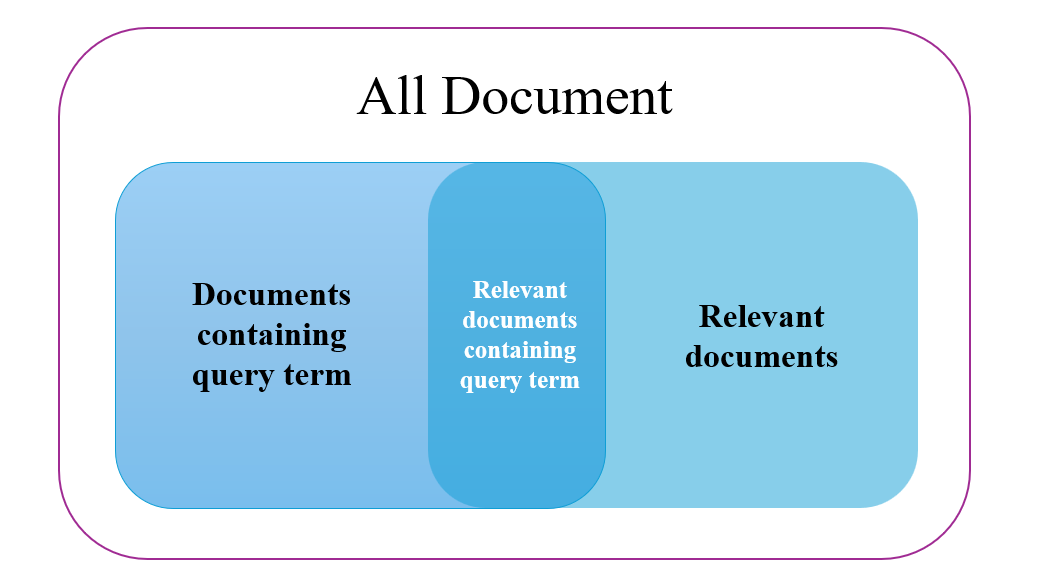
\includegraphics[width=0.8\textwidth]{Images/Related work and tool/BM25.png}
    \vspace{3mm}
    \caption{BM25 visualization.}
    \end{figure}

\textbf{Dense Retrieval Methods}: Leveraging semantic embeddings, dense retrieval tools like SBERT \cite{reimers-2019-sentence-bert}'s Semantic Search and approximate techniques (e.g., HNSW \cite{malkov2018hnsw}, ANNOY \cite{bernhardsson_annoy}, and LSH \cite{jafari2021lsh}) provide scalable solutions for large knowledge bases. These approaches achieve significant speed improvements with minimal accuracy trade-offs \cite{he2024}.
    
    % \begin{figure}[H]
    % \centering
    % 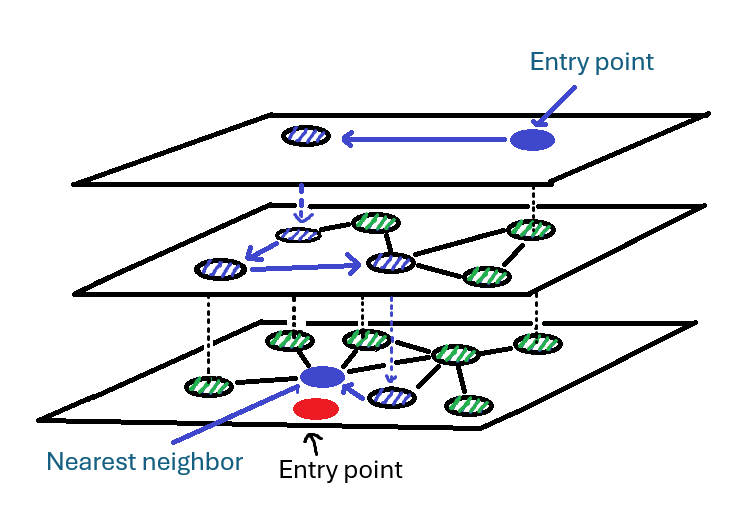
\includegraphics[width=0.8\textwidth]{Images/Related work and tool/HNSW.png}
    % \vspace{3mm}
    % \caption{HNSW visualization.}
    % \end{figure}

    \begin{figure}[H]
    \centering
    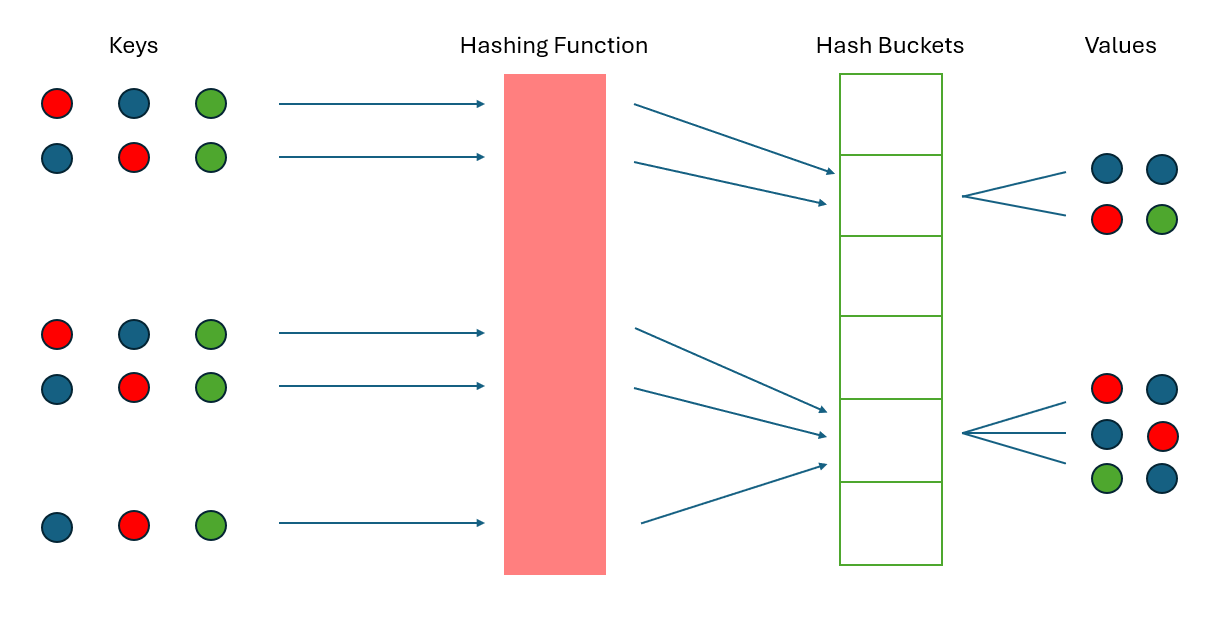
\includegraphics[width=0.8\textwidth]{Images/Related work and tool/LSH.png}
    \vspace{3mm}
    \caption{LSH visualization.}
    \end{figure}
    
\textbf{Selective Retrieval}: Frameworks such as Repoformer \cite{wu2024} employ selective retrieval, determining the necessity of retrieval based on contextual evaluation. This approach reduces inefficiencies and avoid adding irrelevant context.

    \begin{figure}[H]
    \centering
    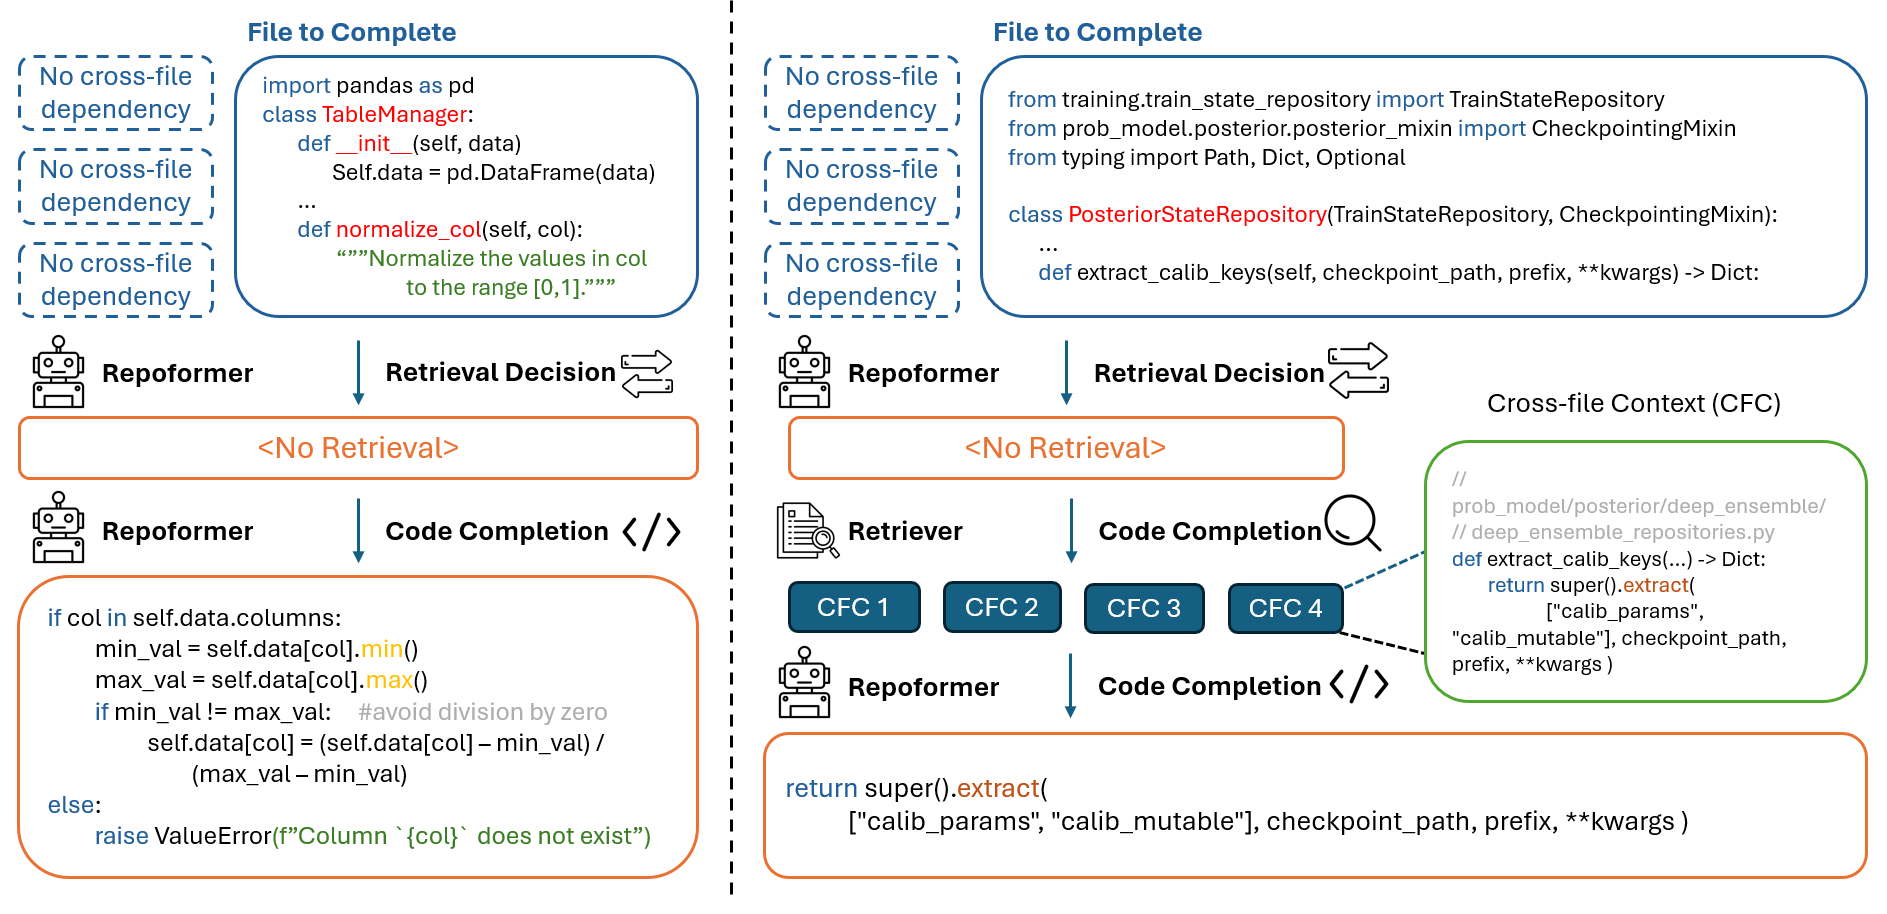
\includegraphics[width=1\textwidth]{Images/Related work and tool/Repoformer.png}
    \vspace{3mm}
    \caption{REPOFORMER framework \cite{wu2024}.}
    \end{figure}
    
\textbf{Multi-Retrieval Perspectives}: Systems like ProCC \cite{tan2024} utilize diverse perspectives, including lexical semantics, hypothetical line embeddings, and code summarization, to enrich context and improve code completion accuracy.

    \begin{figure}[H]
    \centering
    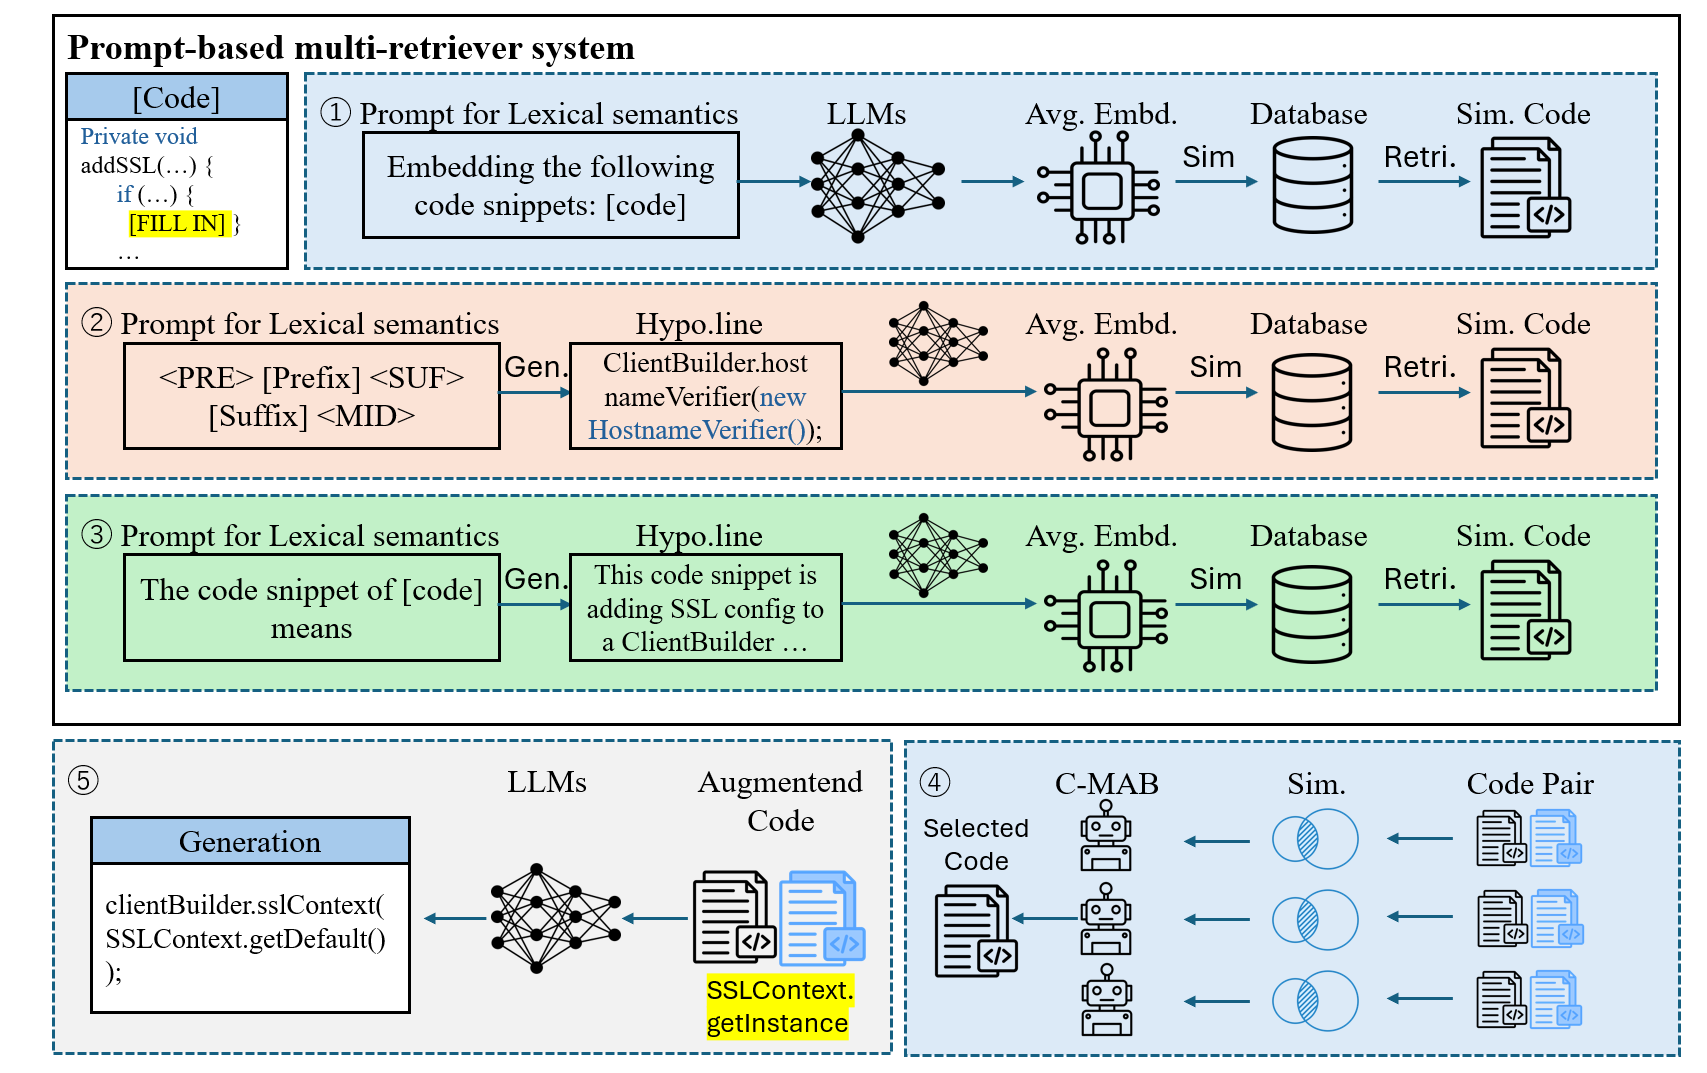
\includegraphics[width=1\textwidth]{Images/Related work and tool/ProCC.png}
    \vspace{3mm}
    \caption{ProCC framework \cite{tan2024}.}
    \end{figure}
    
    \textbf{Multilingual and Multifunctional Embeddings}:
    Models like BGE M3-Embedding \cite{chen2024bge} support over 100 languages and various retrieval functionalities, including dense, multi-vector, and sparse retrieval, enhacing versatility in coding tasks.

    \begin{figure}[H]
    \centering
    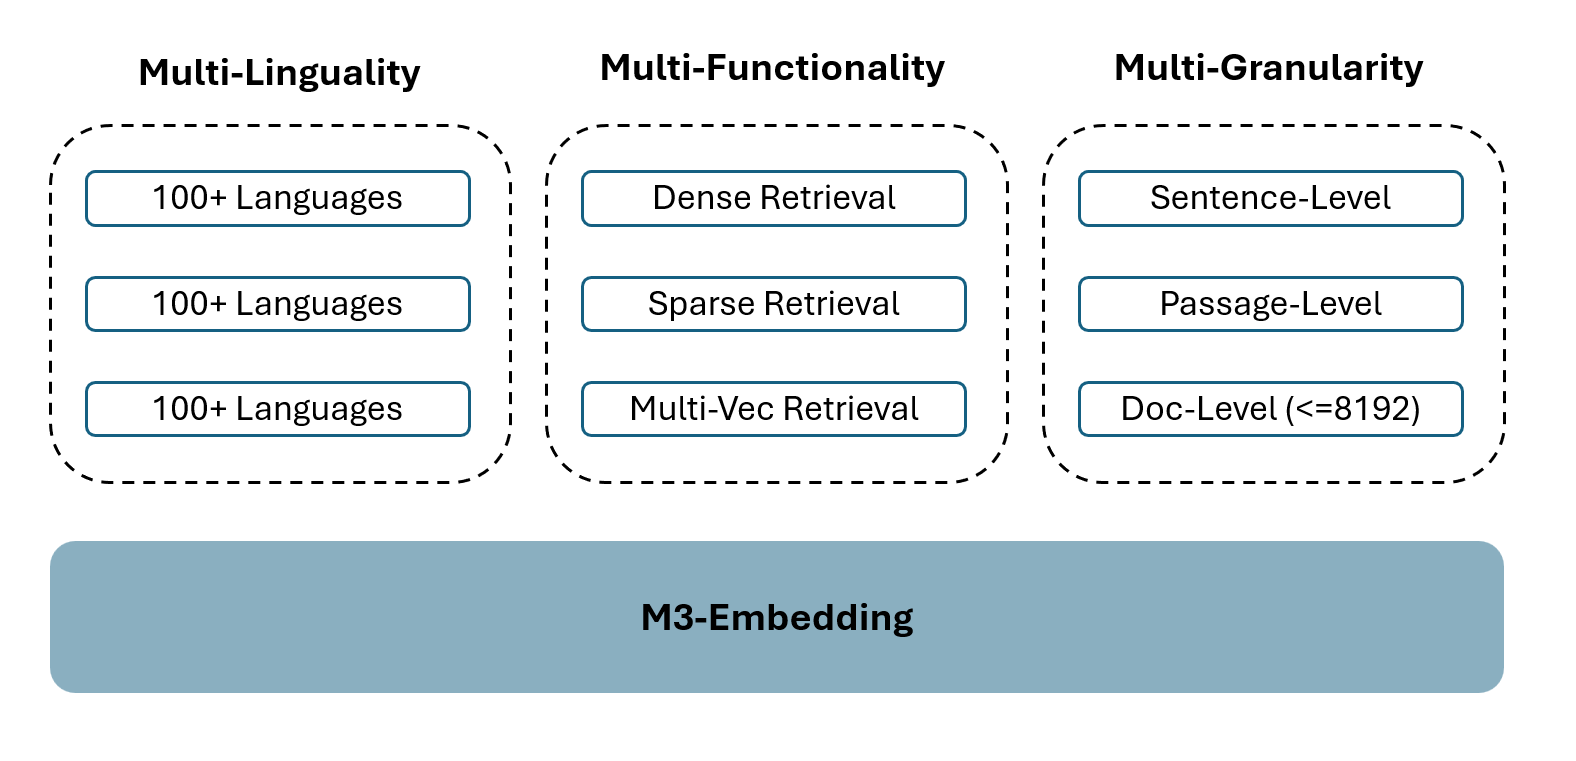
\includegraphics[width=1\textwidth]{Images/Related work and tool/Characters of M3-Embedding.png}
    \caption{Characters of M3-Embedding \cite{chen2024bge}.}
    \end{figure}

\subsection{Generative Enhancements}

\textbf{Generative Pre-trained Transformers}: LLMs like GPT-2 \cite{radford2019} and Code Llama \cite{roziere2023code} are trained on extensive code corpora, enabling them to handle diverse tasks such as function completion and API usage.

    \begin{figure}[H]
    \centering
    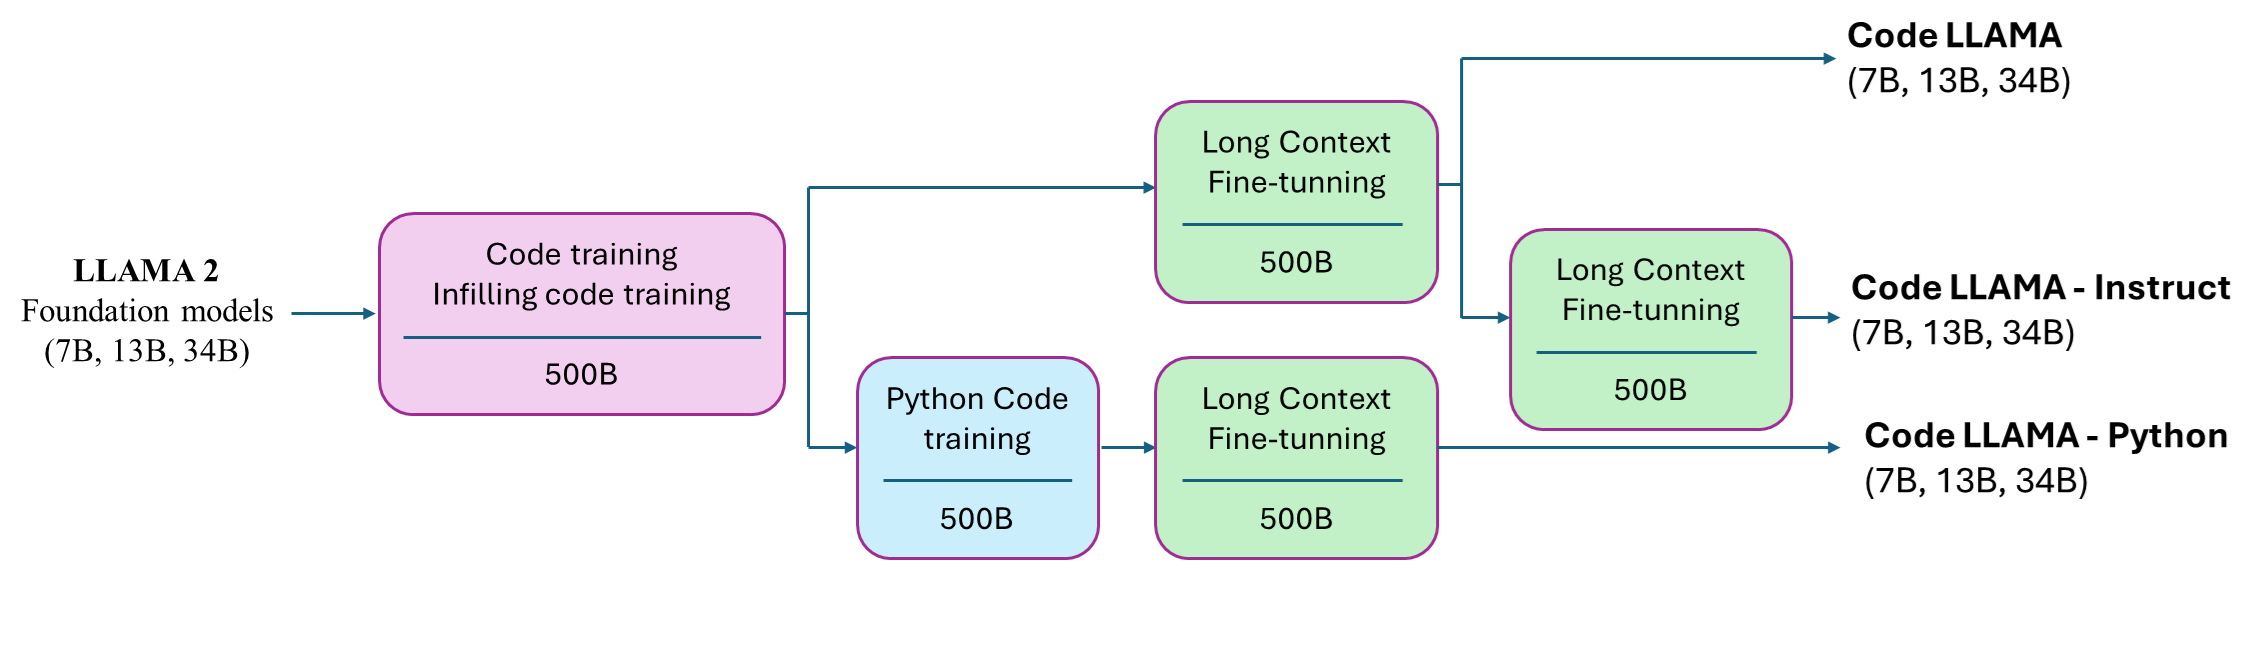
\includegraphics[width=1\textwidth]{Images/Related work and tool/llama2.png}
    \caption{The Code Llama specialization pipeline \cite{roziere2023code}.}
    \end{figure}
    
\textbf{In-Context Augmentation}: RAG pipelines integrate retrieved code snippets directly into prompts, enhancing generation without additional fine-tuning. This approach is particularly effective for repository-level code generation \cite{hostnik2024}.

    \begin{figure}[H]
    \centering
    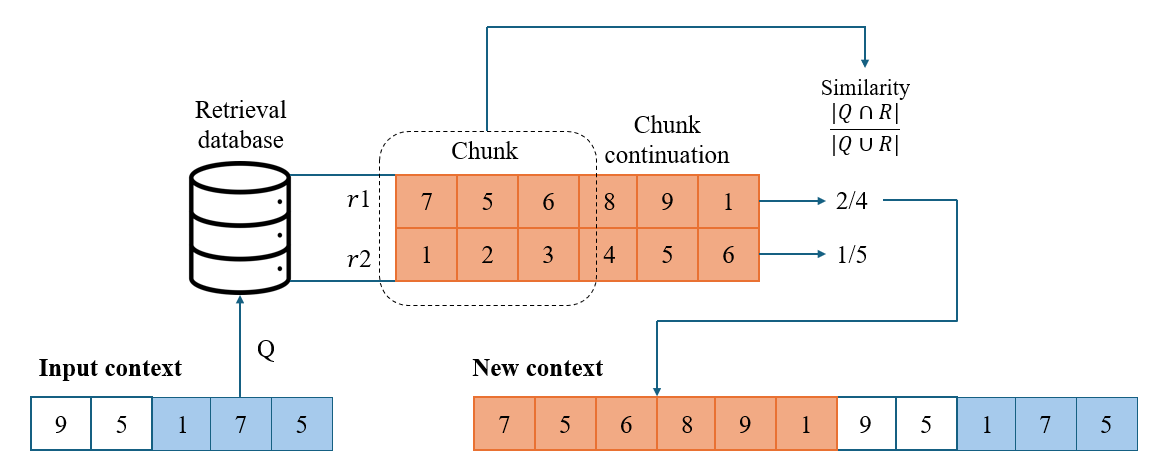
\includegraphics[width=1\textwidth]{Images/Related work and tool/snippet additional metadata.png}
    \vspace{2mm}
    \caption{The retrieved snippet contains continuation tokens and additional metadata \cite{hostnik2024}.}
    \end{figure}
    
\textbf{Specialized Models for Coding}: Models like Qwen2.5-Coder \cite{hui2024qwen2.5} and CodeQwen1.5-7B-Chat \cite{bai2023qwen} are fine-tuned for coding tasks, demonstrating improved performance in code generation and comprehension.

    \begin{figure}[H]
    \centering
    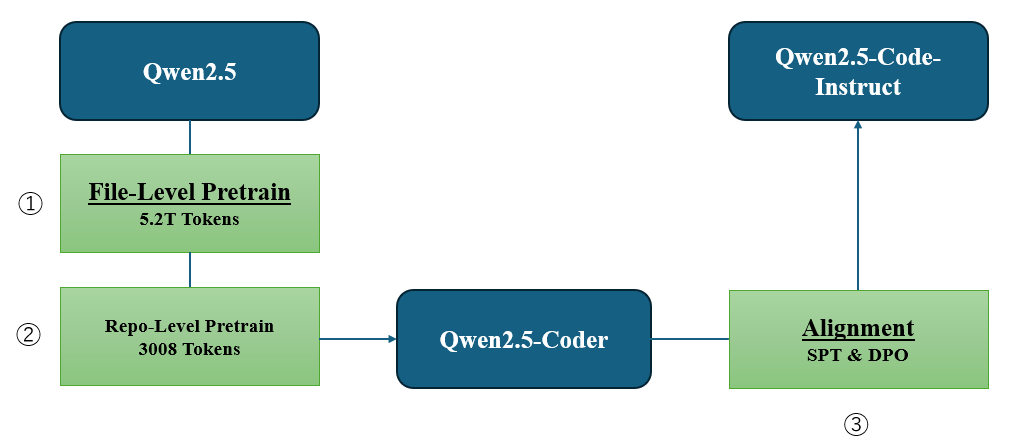
\includegraphics[width=1\textwidth]{Images/Related work and tool/The three-stage training pipeline for Qwen2.5-Coder.png}
    \vspace{2mm}
    \caption{The three-stage training pipeline for Qwen2.5-Coder \cite{hostnik2024}.}
    \end{figure}

\subsection{Specialized Applications}

\textbf{Repository-Level Code Completion}: Tools like Repoformer and RepoCoder \cite{zhang2023repocoder} focus on cross-file dependencies, retrieving and integrating relevant code snippets to improve repository-wide coherence.

    \begin{figure}[H]
    \centering
    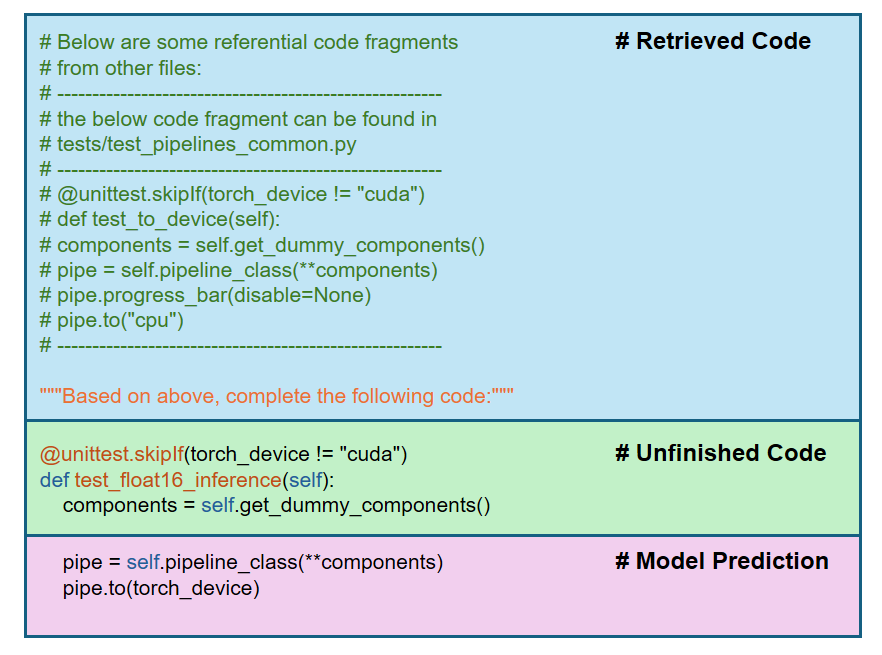
\includegraphics[width=0.8\textwidth]{Images/Related work and tool/RepoCoder.png}
    \vspace{2mm}
    \caption{Demonstrating the format of the RepoCoder prompt \cite{zhang2023repocoder}.}
    \end{figure}
    
\textbf{Commit Message and Assertion Generation}: RAG systems generate commit messages and assertions by retrieving semantically aligned examples, balancing efficiency and effectiveness \cite{he2024}.

\textbf{Code Hallucination Mitigation}: Automated code generation, powered by LLMs, has significantly enhanced development efficiency by generating code from input requirements. However, LLMs often produce hallucinations, particularly when handling complex contextual dependencies in repository-level development scenarios. To address these challenges, RAG-based mitigation methods have been proposed \cite{zhang2024}.

\section{Developer Assistance Tools}

\subsection{Functionality}

\textbf{Search and Retrieval Tools}: Platforms like Stack Overflow\footnote{\href{https://stackoverflow.com/}{Stack Overflow - https://stackoverflow.com/}} provide a database of Q\&A posts where users search for solutions based on keywords or queries. Neural Code Search (NCS) \cite{sachdev2018} enhances this by enabling natrual language queries over raw codebases without curated answers, using vector embeddings and ranking strategies.

    \begin{figure}[H]
    \centering
    
\includegraphics[width=1\textwidth]{Images/Related work and tool/stackoverflow-trends-chart.png}
    \vspace{1mm}
    \caption{Stackoverflow trends chart 2008-2024.}
    \end{figure}

    \begin{figure}[H]
    \centering
    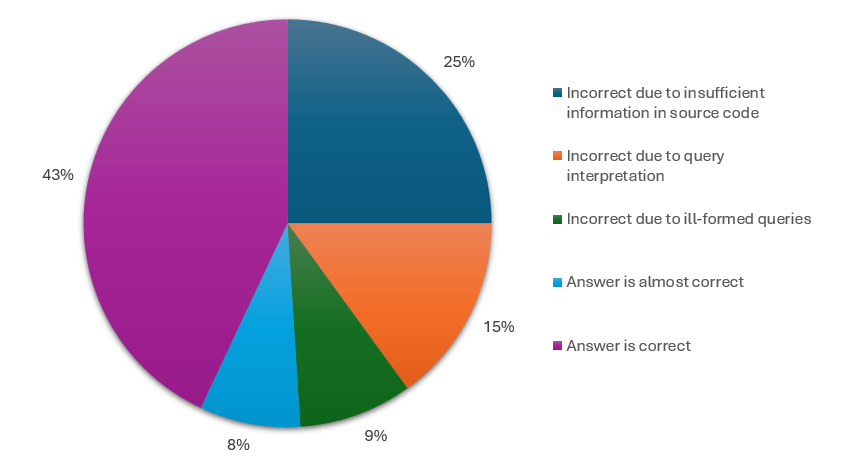
\includegraphics[width=0.9\textwidth]{Images/Related work and tool/NCS evaluation results.png}
    \vspace{3mm}
    \caption{NCS evaluation results \cite{sachdev2018}.}
    \end{figure}
    
\textbf{Code Completion and Suggestion Systems}: Intelligent tools like IntelliCode Compose \cite{svyatkovskiy2020} and example-based systems \cite{bruch2009} prioritize providing relevant suggestions for method calls, arguments, and entire lines of code. These systems are designed to enhance developer productivity by learning from existing codebases.

\textbf{Hybrid Generation Systems}: RAG models combine retrieval with generative capabilities \cite{lewis2020}, producing specific and contextually appropriate outputs by accessing external document repositories and leveraging models

\subsection{Retrieval Mechanisms}
\textbf{Keyword-Based Retrieval}: Traditional forums rely on keyword searches, often yielding broad results with low contextual relevance.

\textbf{Embedding-Based Retrieval}: Tools like NCS employ word embeddings, TF-IDF weighting \cite{mitra2017}, and vector similarity for precise retrieval of relevant code snippets. These systems also incorporate syntactic and semantic elements extracted from source code.

\textbf{Rule-Based Retrieval}: Example-based systems mine patterns and associations (e.g., frequent co-occurrence of API calls) from repositories to recommend contextually relevant options.

\subsection{Code Generation Capabilities}
\textbf{Static Suggestion Systems}: Earlier systems \cite{bruch2009} relied solely on static type information, offering alphabetically sorted method recommendations without understanding contextual relevance.

\textbf{Generative Models}: IntelliCode Compose represents a generative approach, using transformer-based architectures \cite{vaswani2017} like GPT-C to predict and generate entire lines or blocks of syntactically correct code. This includes multilingual support and optimized decoding methods like beam search.

\subsection{Integration in Development Processes}
\textbf{Standalone Search Interfaces}:
    \begin{itemize}
        \item \textbf{NCS} \cite{sachdev2018}: Functions as an external platform where developers input natural language queries to retrieve relevant code snippets directly from large codebases.
        \item \textbf{Sourcegraph}\footnote{\href{https://sourcegraph.com/}{Sourcegraph - https://sourcegraph.com/}}: Provides a universal code search and navigation tool, enabling developers to search across multiple repositories and languages from a centralized interface.
        \item \textbf{Krugle}\footnote{\href{https://www.krugle.com/}{Krugle - https://www.krugle.com/}}: A specialized search engine designed for searching open-source and enterprise code repositories. It indexes and organizes code by context, allowing developers to locate relevant examples, API usage, and documentation efficiently.
    \end{itemize}

    \begin{table}[h!]
    \centering
    \begin{tabular}{p{3cm}p{4cm}p{4cm}p{4cm}}
    \hline
    \textbf{Feature} & \textbf{NCS} & \textbf{Sourcegraph} & \textbf{Krugle} \\ \hline
    
    \textbf{Functionality}
    & Retrieves code snippets from large codebases using natural language queries.
    & Provides universal code search and navigation across multiple repositories and languages.
    & Searches open-source and enterprise code repositories, indexing code by context. \\ \hline
    
    \textbf{Search Methodology}
    & Maps natural language queries and code snippets into a shared vector space using neural networks.
    & Offers structural code search, matching nested expressions and code blocks beyond regular expressions.
    & Indexes code with advanced filtering for examples, API usage, and documentation. \\ \hline
    
    \textbf{Supported Languages}
    & Initially focused on Java.
    & Supports over 30 programming languages.
    & Supports multiple programming languages. \\ \hline
    
    \textbf{Deployment Options}
    & Research project with datasets available for evaluation.
    & Offers self-hosted solutions via Docker Compose and Kubernetes, as well as a managed cloud service.
    & Web-based platform. \\ \hline
    
    \end{tabular}
    \caption{Comparison of Neural Code Search (NCS), Sourcegraph, and Krugle}
    \end{table}

\textbf{IDE-Embedded Assistance}:
    \begin{itemize}
        \item \textbf{IntelliCode Compose} \cite{svyatkovskiy2020}: Integrates into VSCode, offering real-time code generation and suggestions.
        \item \textbf{Github Copilot}\footnote{\href{https://github.com/features/copilot}{Github Copilot - https://github.com/features/copilot}}: Embedded within various IDEs, including VSCode and JetBrains, it leverages AI to provide code completions and suggestions based on the current context.
        \item \textbf{Tabnine}\footnote{\href{https://www.tabnine.com/}{Tabnine - https://www.tabnine.com/}}: An AI-powered code completion tool that integrates with various IDEs, offering whole-line and full-function code completions based on the current code context.
    \end{itemize}

    \begin{table}[h!]
    \centering
    \begin{tabular}{p{3cm}p{4cm}p{4cm}p{4cm}}
    \hline
    \textbf{Feature} & \textbf{IntelliCode Compose} & \textbf{GitHub Copilot} & \textbf{Tabnine} \\ \hline
    
    \textbf{Functionality} 
    & Provides real-time code generation and suggestions within VSCode.
    & Offers AI-driven code completions and suggestions across various IDEs.
    & Delivers whole-line and full-function code completions based on current code context. \\ \hline
    
    \textbf{Supported IDEs}
    & VSCode.
    & VSCode, JetBrains suite, Neovim, and others.
    & VSCode, IntelliJ IDEA, Sublime Text, Atom, and more. \\ \hline
    
    \textbf{AI Model}
    & Utilizes machine learning models trained on open-source GitHub repositories.
    & Powered by OpenAI's Codex model, trained on a vast dataset of public code.
    & Employs proprietary models trained on permissively licensed open-source code. \\ \hline
    
    \textbf{Privacy and Security}
    & Processes code locally, enhancing privacy.
    & Processes code in the cloud, which may raise privacy concerns for sensitive codebases.
    & Offers both cloud-based and on-premises solutions, with options for local processing to ensure code privacy. \\ \hline
    
    \textbf{Pricing}
    & Included with VSCode.
    & Individual model: \$10/month; Business version at \$19/month and Enterprise at \$39/user/month
    & Basic model: free version with basic features; Dev version at \$9/month and Enterprise at \$39/user/month \\ \hline
    
    \end{tabular}
    \caption{Comparison of IntelliCode Compose, GitHub Copilot, and Tabnine}
    \end{table}

\begin{figure}[H]
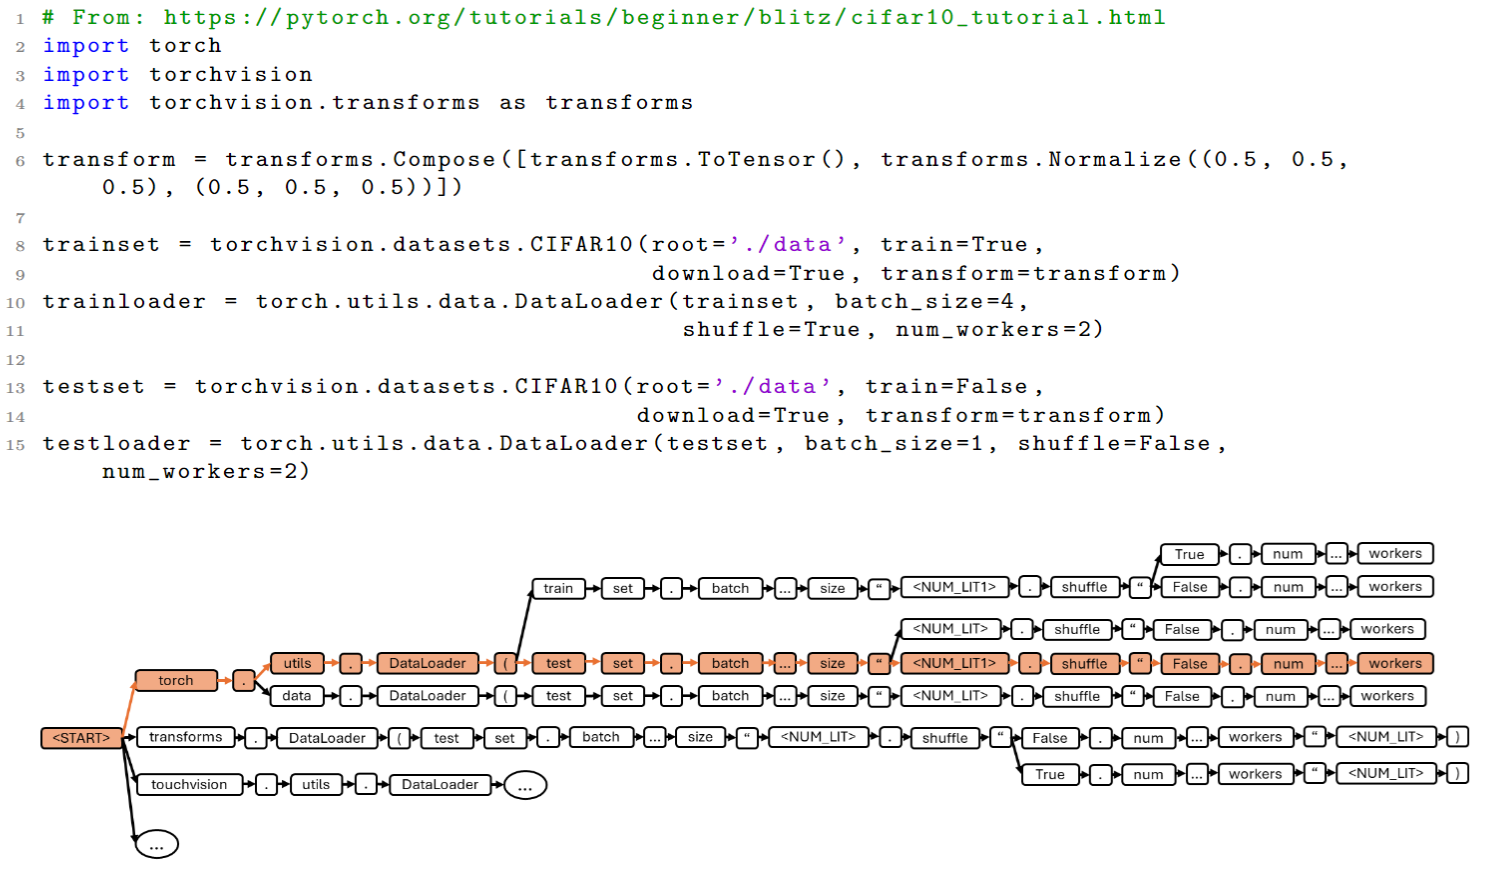
\includegraphics[width=1.05\textwidth]{Images/Related work and tool/Code Snippet and Completion suggestion.png}
\vspace{3mm}
\caption{Code Snippet and Completion suggestion}
\end{figure}